
\documentclass[tikz]{standalone}
\usepackage{tikz}
\begin{document}

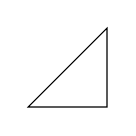
\begin{tikzpicture}
\draw (0, 0) -- (1, 0) -- (1, 1) --cycle;
\end{tikzpicture}
\tikz \draw[thick,rounded corners=20pt] (0,0) -- (0,2) -- (1,3.25) -- (2,2) -- (2,0) -- (0,2) -- (2,2) -- (0,0) -- (2,0);
\begin{tikzpicture}
\draw (-1.5,0) -- (1.5,0);
\draw (0,-1.5) -- (0,1.5);
\draw (-1,0) .. controls (-1,0.555) and (-0.555,1) .. (0,1)
.. controls (0.555,1) and (1,0.555) .. (1,0);
\end{tikzpicture}

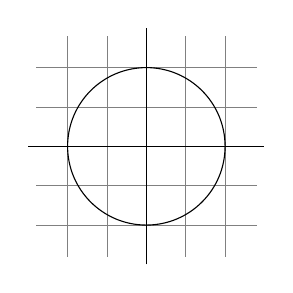
\begin{tikzpicture}
\draw[step=0.5cm,gray,very thin] (-1.4,-1.4) grid (1.4,1.4);
\draw (-1.5,0) -- (1.5,0);
\draw (0,-1.5) -- (0,1.5);
\draw (0,0) circle [radius=1cm];
\end{tikzpicture}

\begin{tikzpicture}
[Karl’s grid/.style ={help lines,color=#1!50},
Karl’s grid/.default=blue]
\draw[Karl’s grid]
(0,0) grid (1.5,2);
\draw[Karl’s grid=red] (2,0) grid (3.5,2);
\end{tikzpicture}
\end{document}